% Report
\documentclass{article}

% Here set the various packages
% Packages to load
\usepackage[english]{babel}
% %%% Support some german text
% \usepackage{ngerman}
% \usepackage[latin1]{inputenc}   % für Umlaute
%%%
% \usepackage[utf8]{inputenc}
\usepackage[T1]{fontenc}
\usepackage{microtype}

%%%
% \usepackage[inline]{enumitem} % Required for the "description" list.

%%% Fix for not hyperlinking citations
\makeatletter
\let\NAT@parse\undefined
\makeatother
\usepackage{hyperref}
% 
\usepackage{cite}
% \ifx\pdfoutput\undefined
% 	\usepackage{graphicx}
% \else
% 	\usepackage[pdftex]{graphicx}
% \fi
\usepackage{graphicx}
\graphicspath{{Figures/}}
\usepackage{amsmath}
% \interdisplaylinepenalty=2500

% Shading of questions. Use the "shaded" environment or the "\hl{}" command.
\usepackage{framed}
% \usepackage[dvipsnames]{color}
\usepackage[svgnames]{xcolor}
\usepackage{soul}
% Nice colours: Gainsboro, LightGoldenrod, LightSteelBlue
% furter ref: https://www.latextemplates.com/svgnames-colors
\definecolor{shadecolor}{named}{Gainsboro}
\sethlcolor{Gainsboro}

%%% Todo margin notes (enable/disable)
\usepackage{todonotes}
% \usepackage[disable]{todonotes}
%%%

%eof

%%%

\title{Programming of Supercomputers\\Worksheet 1}
\author{
	Oleksandr Voloshyn \texttt{<o.voloshyn@tum.de>}\\ 
	Qunsheng Huang \texttt{<keefe.huang@tum.de>}\\ 
	Tommaso Bianucci \texttt{<bianucci@in.tum.de>}
	}
\date{\today}

\begin{document}

\maketitle
\renewcommand{\abstractname}{Group members's contributions}
\begin{abstract}
	\begin{center}
	% Here write the contributions of the members of the group
	Oleksandr Voloshyn: worked on 4.1, 4.2, 4.3, 5.1, 5.3

	Tommaso Bianucci: worked on 4.1, 4.2, 4.3, 5.2, 5.3
	
	Qunsheng Huang: worked on 4.1, 4.3, 4.4, 5.1
	\end{center}
\end{abstract}

\section{Performance baseline} % Name of assignment 1
\subsection{GNU Profiler} % Name of sub-assignment
% \subsubsection{Questions}
\begin{enumerate}
	\item \hl{Which routines took 80\% or more of the execution time of the benchmark?}

	\begin{enumerate}
		\item Serial
		\begin{itemize}
			\item EvalEOSForElems(Domain\&, double*, int, int*, int) --- 28.18\%
			\item CalcHourglassControlForElems(Domain\&, double*, double) --- 17.10\% 
			\item CalcFBHourglassForceForElems(...) --- 15.76\%
			\item CalcKinematicsForElems(Domain\&, double, int) --- 11.84\%
			\item IntegrateStressForElems(Domain\&, double*, double*, double*, double*, int, int) --- 10.98\%
		\end{itemize}
		These functions account for 83.86\% of total execution time.

		\item OpenMP
		\begin{itemize}
			\item CalcHourglassControlForElems(Domain\&, double*, double) --- 29.90\%
			\item ApplyMaterialPropertiesForElems(Domain\&) --- 22.58\%
			\item CalcFBHourglassForceForElems(...) --- 15.84\%
			\item IntegrateStressForElems(...) --- 14.28\%
		\end{itemize}
		These functions account for 82.60\% of total execution time.
		\vspace{1mm}

		\item MPI
		\begin{itemize}
			\item EvalEOSForElems(Domain\&, double*, int, int*, int) --- 24.44\%
			\item LagrangeNodal(Domain\&) --- 21.86\%
			\item CalcFBHourglassForceForElems(..) --- 16.67\%
			\item CalcKinematicsForElems(Domain\&, double, int) --- 11.12\%
			\item IntegrateStressForElems(...) --- 10.15\%
		\end{itemize}
		These functions account for 84.24\% of total execution time.

		\item Hybrid
		\begin{itemize}
			\item CalcFBHourglassForceForElems(..) --- 23.05\%
			\item EvalEOSForElems(Domain\&, double*, int, int*, int) --- 21.22\%
			\item LagrangeNodal(Domain\&) --- 18.95\%
			\item IntegrateStressForElems(...) --- 13.02\%
			\item CalcKinematicsForElems(Domain\&, double, int) --- 10.29\%
		\end{itemize}
		These functions account for 86.53\% of total execution time.
	\end{enumerate}

	\item \hl{Is the measured execution time of the application affected by gprof? \\Hint: use the time command to determine this.}

	The measured execution time does not differ with use of gprof. This was tested with the four benchmarks with the following results:
	\begin{center}
		\begin{tabular}{|c|c|c|}
			\hline
			&Time without Gprof (s) & Time with Gprof (s)\\
			\hline
			Serial &53.90&53.88\\ \hline
			OpenMP &21.06&20.95\\ \hline
			MPI &120.78&120.84\\ \hline
			Hybrid &46.9&45.95\\ \hline
		\end{tabular}
	\end{center}
	Each benchmark was run 2-3 times with and without gprof. The times did vary slightly but indicated that the usage of gprof did not change th execution time. The results in the above table can be seen in the attached gprof files.

	\item \hl{Can gprof analyze the loops (for, while, do-while, etc.) of the application?}

	No, gprof cannot be used to analyse loops.
	
	\item \hl{Is gprof capable of analyzing parallel applications?}

	Yes, gprof can be used to analyse some parallel applications. However, typically only the performance of the main thread is recorded (as in the case of MPI implementations). The obscuring of information can be seen especially in the case of openMP, where the code spends more than 50\% of the time in "frame dummy", a function that does not exist in source code.

	\item \hl{What is necessary to analyze parallel applications?}

	Gprof typically only produces one \verb!gmon.out! output file for the main process. However, in a parallel process, multiple output files are required. When using MPI processes, it is possible to inform gprof, via environmental variables, of the number of threads produced and run. One \verb!gmon.out! is then produced per thread. These files can then be aggregated to determine the overall behavior of all threads together or analysed separately.

	\item \hl{Where there performance differences between the GNU++ and the Intel compiler?}

	There were differences between the two compilers. In general, the code compiled by the Intel compiler was slightly faster. The difference between the code compiled by the two compilers is approximately 2s and this varied slightly each job. Four jobs were run using the automated script in Section 4.2 of the assignment - in both cases, the Intel compiled code ran approximately ~2s faster with the optimal.
\end{enumerate}

\subsection{Compiler flags}
\begin{enumerate}
	\item \hl{Look at the compilers help (by issuing icc -help and gcc -help). How many opti-
	mization flags are available for each compiler (approximately)?}

	gcc-help shows approximately 100 compiler flags, icpc-help show approximately 18 optimization flags, 8 interprocedural optimization flags, 60 advanced optimization options and 20 profile guided optimizations, for a total of 106 flags.

	\item \hl{Given how much time it takes to evaluate a combination of compiler flags, is it realistic to test all possible combinations of available compiler flags? What could be a possible solution?}

	Each test run takes approximately 40-50 seconds to complete, excluding the time required for compilation of the code. Given that there are more than 100 optimization flags for each compiler, we can conservatively estimate that the total time to completion would exceed $6\times10^{32}s$, which is completely unfeasible. Instead, it would make sense for us to examine the code to determine what possible bottlenecks exist and apply flags that could improve the situation.

	\item \hl{Which compiler and optimization flags combination produced the fastest binary?}

	For the GNU++ compiler, we determined that the effect of the flags was somewhat inconsistent. We performed a simple statistical analysis of the effects of the flags over 3 runs. Overall, we observed that the flags "-march=native" and "-funroll-loops" were constantly associated with binaries with the best performance.

	For the Intel compiler, the fastest binary only used "-unroll" flag with a time of 50.43s to completion with a speedup of 1.00258. The second fastest binary was without flags with a time of 50.56.

	The fastest binary from both compilers was compiled using the Intel compiler with the "-unroll" flag.
\end{enumerate}

\subsection{Optimization pragmas}
\begin{enumerate}
	\item \hl{What is the difference between Intel's \emph{simd}, \emph{vector} and \emph{ivdep} \emph{\#pragma} directives?}

	The three pragmas allow the compiler to ignore certain requirements when vectorizing. The simd pragma forces vectorization to occur, ignoring safety or cost. The vector pragma forces the compiler to ignore cost when deciding to vectorize (as a result the code may run slower after vectorization). The ivdep pragma instructs compiler to ignore assumed vector dependencies - ie compiler may choose to treat assumed dependencies as proven dependencies. This pragma instructs compiler to ignore such assumptions and proceed with vectorisation.
	\item \hl{Why did you choose to apply the selected \#pragma in the particular location?}

	We chose to apply \verb!#pragma loop_count avg(27000)! to the function \verb!CalcHourglassControlForElems! in lulesh.cc. When running the task in serial, more than 70\% of overall runtime time was spent in this function. This function contains a highly complicated loop that may require specific treatment for optimization.
\end{enumerate}

\subsection{Inline assembler}
\begin{enumerate}
	\item \hl{Is the inline assembler necessarily faster than compiler generated code?}

	Not necessarily. The speed increase is dependent on the implementation on the code - especially when modern compilers already implement many forms of optimization. It is often likely that hand-written assembler code is often slower than compiler optimized assembler code. However, there do exist specific cases where an inline assembler may be faster. The most relevant cases to this module include:
	\begin{itemize}
		\item \hl{Implement instructions which are not yet possible in the current language. For example, certain operations, such as a full-multiplication operator in C---2N-bit result from N-bit inputs. Most x86 CPUs can, however, perform this operation in a single instruction. In these rare cases, it would be beneficial to use optimal functions that belong to the specific CPU when available.}

		\item \hl{Spot-optimizing specific lines of code. For example, compilers may not optimally vectorize complicated loops, since it has to deal with many general cases. If the programmer understands the problem well, it may be beneficial to use the inline assembler to perform the loop operations.}
	\end{itemize}
	
	\item \hl{On the release of a CPU with new instructions, can you use an inline assembler to take advantage of these instructions if the compiler does not support them yet?}

	Yes. One benefit to inline assemblers is that it allows access to processor specific instructions which the compiler may not support. Examples may include FPU instructions that may be faster than compiler generated floating operations. However, the onus of correct usage of these commands then falls on the programmer.
	
	\item \hl{What is AVX-512? Which CPUs support it? Is there any compiler or language support for these instructions at this moment?}

	AVX stands for Advanced Vector Extensions SIMD instructions. AVX-512 are the 512-bit extensions to the preexisting AVX/AVX2 instructions. They were first supported by the Xeon-Phi x200 (Knights Landing) and Skylake-X CPUs. Note that AVX-512 is not the first 512-bit SIMD instructions released by Intel. These commands are supported in the intel C++ compiler under the namespace AVX. The \verb!-xCOMMON-AVX512! flag can be used for auto-vectorization using AVX-512 functions.
\end{enumerate}

% Figure example
%\begin{figure}[h!] % h=here, t=top, b=bottom, p=(extra)page, !=force
 %	\begin{center}
 %		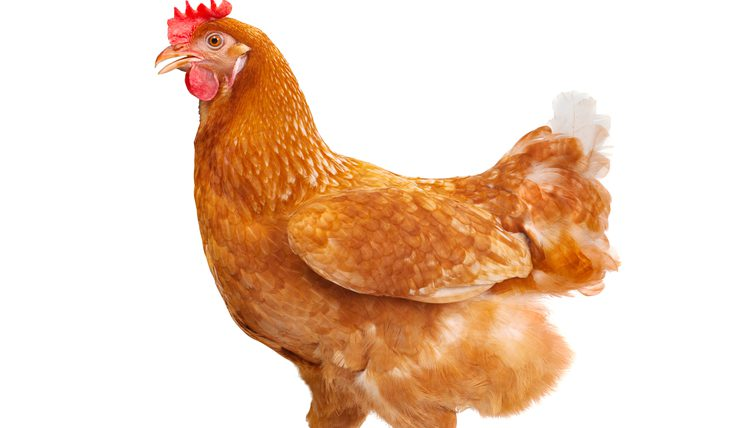
\includegraphics[width=.9\linewidth]{figure.png} % It searches in the Figures/ folder!
 %		\caption{Caption text}
 %		\label{fig:figureLabelName}
 %	\end{center}
%\end{figure}

\section{Performance Scaling}
\subsection{OpenMP}
\begin{enumerate}
	\item \hl{Was linear scalability achieved?}

	Linear scalability was achieved for certain numbers of processors. For the GNU++ compiler, we see a linear scaling (with regards to speed) if the number of threads is between 1 and 5. We see a similar pattern for the Intel compiler between 1 and 7 threads. These two trends can be seen in Fig. \ref{fig:omp_speedup}. After the maximum speedup is achieved, we then see that speedup decreases sharply and performance worsens. This is especially the case for the Intel compiler---when using more than 26 processors, the speedup drops below 1. 

	% Figure example
	\begin{figure}[h!] % h=here, t=top, b=bottom, p=(extra)page, !=force
	 	\begin{center}
	 		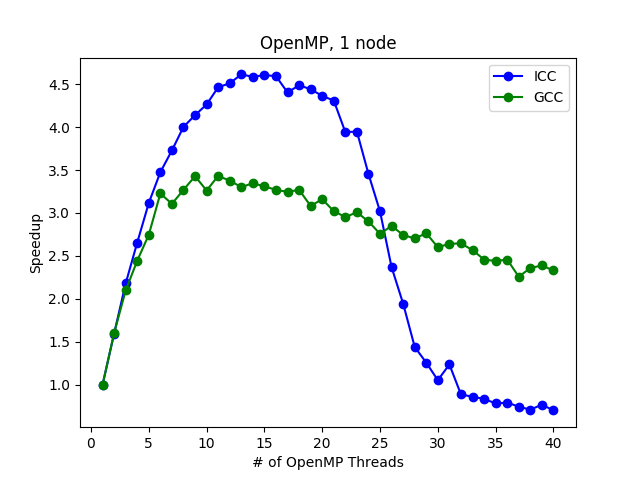
\includegraphics[width=.7\linewidth]{OMP_speedup.png} % It searches in the Figures/ folder!
	 		\caption{OpenMP: Speedup vs. \# Processors}
	 		\label{fig:omp_speedup}
	 	\end{center}
	\end{figure}

	We can also identify a problem when increasing the number of threads while keeping the domain constant - the performance of the program cannot be guaranteed if the domain is too small. We observe sudden decreases in speedup with both compiler above 8 threads (seen as spiky segments along the speedup graph)---this is likely due to issues with non-uniform memory access, especially since there is little transparency or control over how memory is accessed in OpenMP.

	\item \hl{On which thread-count was the maximum performance achieved? Was it the same for both the Intel and the GNU compilers?}

	For the Intel compiler, the maximum speedup was 4.64 (11.32s) with 16 threads. For the GNU++ compiler, the maximum speedup was 3.43 (19.57s) with 15 threads. The minimum point can be seen in Fig \ref{omp_time}. While the Intel compiler experienced the best speedup (and fastest time), the speedup also rapidly decayed after a certain point (at 40 processors, the program took almost 100s to complete). The program compiled by the GNU++ compiler did also see a reduction in speedup but the overall time remained below 30s at 40 processors.
	
		\begin{figure}[h!] % h=here, t=top, b=bottom, p=(extra)page, !=force
	 	\begin{center}
	 		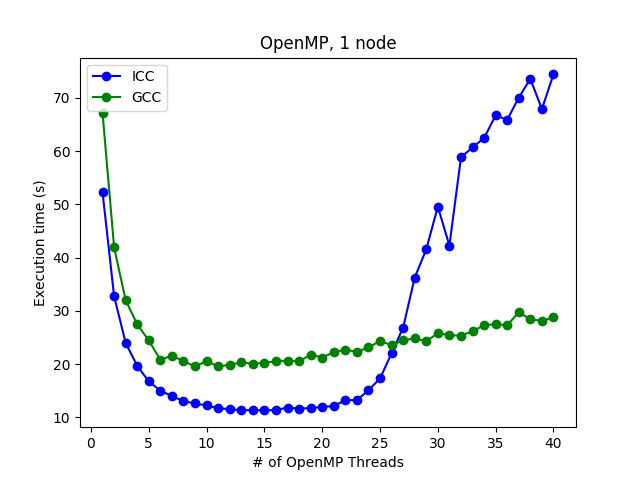
\includegraphics[width=.7\linewidth]{OMP_time.png} % It searches in the Figures/ folder!
	 		\caption{OpenMP: Execution Time vs. \# Processors}
	 		\label{fig:omp_time}
	 	\end{center}
	\end{figure}
	
			\begin{figure}[h!] % h=here, t=top, b=bottom, p=(extra)page, !=force
	 	\begin{center}
	 		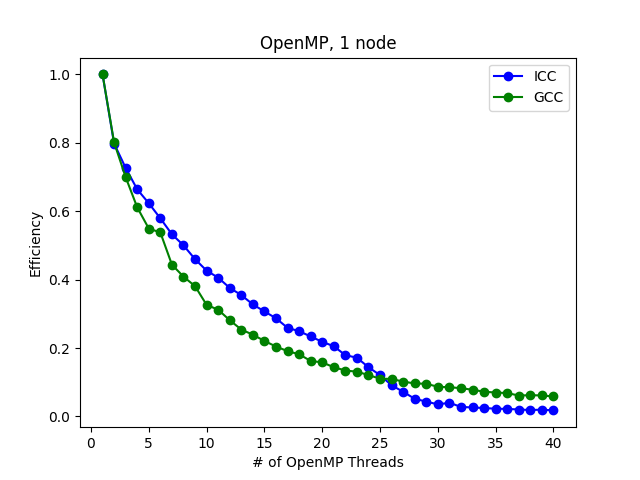
\includegraphics[width=.7\linewidth]{OMP_efficiency.png} % It searches in the Figures/ folder!
	 		\caption{OpenMP: Efficiency vs. \# Processors}
	 		\label{fig:omp_efficiency}
	 	\end{center}
	\end{figure}

\end{enumerate}

\subsection{MPI}
\begin{enumerate}
	\item \hl{What are the valid combinations of processes allowed?}

	Only number of processes which are perfect cubes are allowed. So on a single node, which has 40 cores, we can use 1, 8, 27.
	

	\item \hl{Was linear scalability achieved?}

	% Definitions of strong and weak scaling efficiency from:
	% https://www.sharcnet.ca/help/index.php/Measuring_Parallel_Scaling_Performance

	\begin{description}
		\item[Weak]	 Ideal linear weak scaling occurs when the runtime does not vary with the number of processes. We could instead see (Fig.\ref{fig:MPI_weakScaling}) a marked increase in runtime in this case and the \emph{weak scaling efficiency}\footnote{Defined as $speedup(N) = \frac{T(1)}{T(N)}$ where $N$ is the number of processes.} decreasing drastically.

		\item[Strong]
		Ideal linear strong scaling is achieved if the speedup equals the number of processes, i.e. if $S(N) = N$.

		To test strong scaling we adjusted the problem size per MPI process in order to keep the volume of the entire domain constant. This means that in our test runs with initial size 24, we used $s=24$, $s=12$, $s=8$ for 1, 8 and 27 MPI processes respectively, while for our test runs with initial size 30, we used $s=30$, $s=15$, $s=10$ for 1, 8 and 27 MPI processes respectively.

		We could observe a quite good linear scaling behaviour, although not perfect. As shown in Fig.\ref{fig:MPI_strongScaling}, the actual speedup (solid blue line) quite follows the ideal linear scaling one (dashed red line). The \emph{strong parallel efficiency}\footnote{Defined as $speedup(N)/N = \frac{T(1)}{N \cdot T(N)}$.} drops to $80\%$ with 27 MPI processes on the same node.

		\begin{figure}[p] % h=here, t=top, b=bottom, p=(extra)page, !=force
		 	\begin{center}
		 		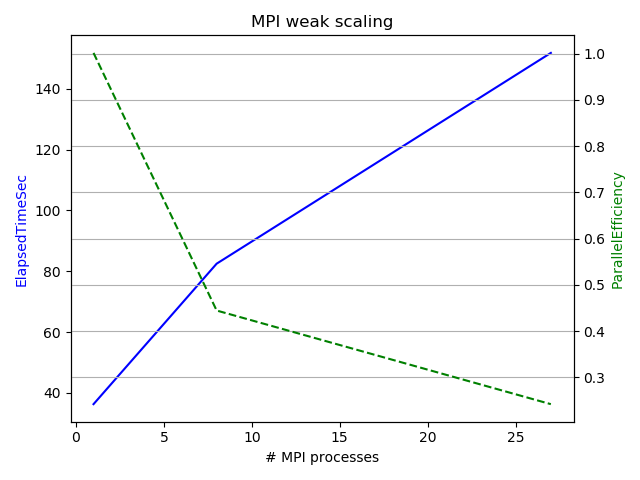
\includegraphics[width=.75\linewidth]{MPI_weak_scaling_all.png} % It searches in the Figures/ folder!
		 		\caption{MPI weak scaling results. Average of $s=24$ and $s=30$.}
		 		\label{fig:MPI_weakScaling}
		 	\end{center}
		\end{figure}
		\begin{figure}[p] % h=here, t=top, b=bottom, p=(extra)page, !=force
		 	\begin{center}
		 		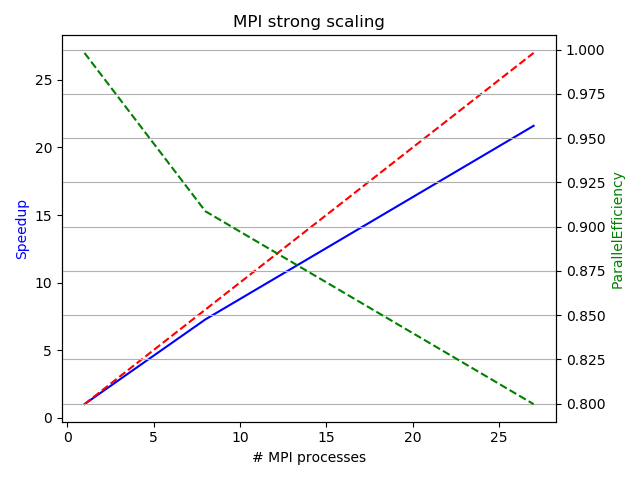
\includegraphics[width=.75\linewidth]{MPI_strong_scaling_all.png} % It searches in the Figures/ folder!
		 		\caption{MPI strong scaling results. Average of $s=24$ and $s=30$.}
		 		\label{fig:MPI_strongScaling}
		 	\end{center}
		\end{figure}
	\end{description}

	\item \hl{On which process-count was the maximum performance achieved?}

	From a strong scaling perspective, the best performance was achieved with 27 MPI processes.

	\item \hl{How does the performance compare to the results achieved with OpenMP in Section 5.1?}

	The results clearly show that using MPI allows for a better strong scaling behaviour compared to OpenMP. With OpenMP we achieve a maximum speedup around 4.5, both with gcc and intel compilers, while with MPI we reach a speedup of 21 with 27 processes.

	TODO
	
	
\end{enumerate}
\subsection{OpenMP + MPI}
\begin{enumerate}
	\item \hl{What are the valid combinations of processes and threads?}

	Understanding that the multiple of MPI processes and OpenMP threads must be less than 40 and that the number of processes must increase in a cubic fashion, we have the following possible combinations for a single node:
	MPI Processes: 8
	OpenMP Threads: 1-5
	
	MPI Processes: 27
	OpenMP Threads: 1
	
	We omit the study of when MPI processes = 1 as the scaling should be identical to the strong scaling in the OpenMP study.
	
	\item \hl{Was linear scalability achieved?}
	
	Weak scaling is achieved when we increase the domain size proportional to the number of processes launched. Currently, if we limit our experiments to a single node, we cannot examine any interesting cases for weak scaling. We would need to keep the number of OpenMP threads per MPI process constant while increasing the domain size to scale with the number of MPI processes. The only possible case would be to examine 1, 8 , and 27 MPI processes with 1 OpenMP thread---the performance is identical to the weak scaling analysed in question 5.2.
	
	Strong scaling is achieved by keeping the problem size constant and increasing the number of threads.This is seen when we run with 8 MPI processes and 1-5 OpenMP threads. 
	
	\begin{description}
		\item[Strong] We ran 2 experiments, one with -s 15 and one with -s 30. We see linear scaling in both cases. However, for the reduced domain size, we see in Fig \ref{fig:hybrid_strongscaling_s15} that the speedup decreases with 5 OpenMP threads. This is expected because, per Amdahl's law, the maximum speedup is limited by problem size. At 5 OpenMP threads, the cost of parallelisation outweights the benefits of parallelisation and we see a decrease in speedup. This can be remedied by increasing the overall domain size. We run the same form of strong scaling with -s=30 in Fig. \ref{fig:hybrid_strongscaling_s30} and we see that speedup continues to increase linearly at 5 OpenMP threads. For the hybrid case, the fastest speedup was for the 
	\end{description}
		
	\begin{figure}[p] % h=here, t=top, b=bottom, p=(extra)page, !=force
	 	\begin{center}
	 		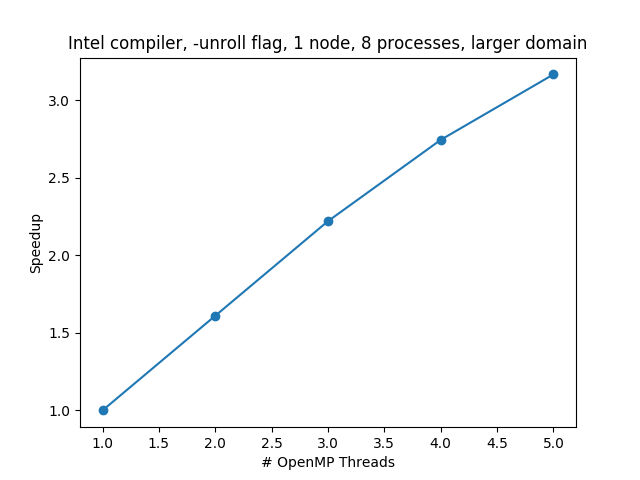
\includegraphics[width=.75\linewidth]{HYBRID_Speedup_30.png} % It searches in the Figures/ folder!
	 		\caption{Hybrid strong scaling, $s=30$.}
	 		\label{fig:hybrid_strongscaling_s30}
	 	\end{center}
	\end{figure}
	
	\item \hl{How does the performance compare to the results achieved with OpenMP in Section 5.1 and with MPI in Section 5.2?}

	We see that the solutions for the hybrid (where number of OpenMP threads and MPI processes are greater than 1) are slower a pure MPI implementation with 27 processes but faster than a pure OpenMP implementation with 15 threads. The fastest speedup was approximately 16.7 times or an elapsed time of 3.75s. 
	
	\item \hl{Which solution is overall the fastest?}

	Overall, the fastest solution is with a pure MPI implementation with a speedup of 21 and a runtime of 2.6 seconds.
	
	\item \hl{Would you have guessed this best combination before performing the experiments in Sections 5.1, 5.2 and 5.3?}

	This is not unexpected. We understand that when running an MPI process, the memory allocation happens separately for each MPI process. However, OpenMP is a form of shared memory parallelisation. As the granularity of the implementation decreases, communication overhead increases for MPI processes, while the costs to maintain memory coherence when multiple threads access similar regions in memory increase for OpenMP processes.
\end{enumerate}

\end{document}

%eof
